\documentclass[unknownkeysallowed, 10pt, a4 paper, handout]{beamer}

% Custom beamer theme
\usepackage{../style/beamerthemeCustom}
\newcommand{\HRule}{\rule{\linewidth}{0.5mm}}   %FOR TITLEPAGE

\usepackage{changepage}       % adjustwidth

\setlength\parskip{0.3cm}

\definecolor{darkgreen}{RGB}{0,100,0}
\newcommand{\green}[1]{\textbf{\textcolor{darkgreen}{#1}}}
\newcommand{\red}[1]{\textbf{\textcolor{red}{#1}}}

\newcommand{\focus}[1]{\textbf{\textcolor{red}{#1}}}
\newcommand{\ra}{$\longrightarrow$ }
\newcommand{\lra}{$\longleftrightarrow$ }

\newcommand{\code}[1]{\colorbox{black}{\color{green}\texttt{#1}}}

% Command to create two side-by-side minipages
\newcommand{\sidebyside}[5]{
  \begin{minipage}{#1\textwidth}
    #2
  \end{minipage} #3 \begin{minipage}{#4\textwidth}
    #5
  \end{minipage}
}

\begin{document}

\begin{frame}
  \begin{center}
    \frametitle{Basic shell scripting}

    As said before, you can \focus{recycle} commands you use more than once:\\
    \focus{write once, use more than once}

    \sidebyside{0.50}{
      You can create \focus{scripts}:\\
      files containing instructions\\
      which you launch to perform tasks
    }{\hfill}{0.45}{
      \begin{center}
        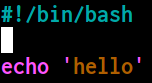
\includegraphics[width=0.70\textwidth]{pics/script_1.png}
      \end{center}
    }

    \begin{itemize}
      \item The first line tells the shell which \focus{interpreter} to use\\
        (i.e. which scripting language, we use \code{bash})
      \item The rest is \focus{instructions} (this here prints 'hello')
    \end{itemize}

    \sidebyside{0.50}{
      Scripts can be made \focus{executable}\\
      (remember \code{chmod}?)\\
      and launched from the command line:\\
      \code{./<script>}
    }{\hfill}{0.45}{
      \begin{center}
        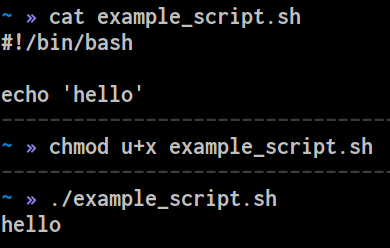
\includegraphics[width=0.80\textwidth]{pics/script_2.png}
      \end{center}
    }
  \end{center}
\end{frame}

\end{document}
